%%%% Paramétrage du TD %%%%
\def\xxactivite{ \ifprof \normalsize{Application 2 -- Corrigé } \else  \ifcolle Colle \else Application 2\fi \fi} % \normalsize \vspace{-.4cm}
\def\xxauteur{\textsl{Xavier Pessoles}}


\def\xxnumchapitre{Chapitre 1 \vspace{.2cm}}
\def\xxchapitre{\hspace{.12cm} Détermination des liaisons équivalentes}


\def\xxcompetences{%
\textsl{%
\textbf{Savoirs et compétences :}\\
\begin{itemize}[label=\ding{112},font=\color{ocre}] 
\item \textit{Mod2.C34} : chaînes de solides.
%\item \textit{Mod2.C34} : degré de mobilité du modèle;
%\item \textit{Mod2.C34} : degré d’hyperstatisme du modèle;
%\item \textit{Mod2.C34.SF1} : déterminer les conditions géométriques associées à l’hyperstatisme;
%\item \textit{Mod2.C34} : résoudre le système associé à la fermeture cinématique et en déduire le degré de mobilité et d’hyperstatisme.
\end{itemize}
}}


\def\xxtitreexo{Tour de la terreur et Mât réacteur}
\def\xxsourceexo{\hspace{.2cm} \footnotesize{F. Weiss \& Éditions Vuibert}}


\def\xxfigures{
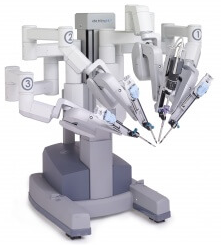
\includegraphics[width=.35\linewidth]{fig_00}
}%figues de la page de garde


\input{\repRel/Style/pagegarde_TD}
\setcounter{numques}{0}
\setlength{\columnseprule}{.1pt}
\pagestyle{fancy}
\thispagestyle{plain}

\vspace{5.2cm}

%%%%%%%%%%%%%%%%%%%%%%%

\setcounter{exo}{0}

\ifprof
\begin{multicols}{2}
\else
\begin{multicols}{2}
\fi


 \ifprof
 \else
 
\subsection*{Ascenseur de la Tour de la terreur\footnote{D'après concours X-ENS PSI.}}% }

La Tour de la terreur du parc Walt Disney Studios propose aux visiteurs d'entrer dans une tour et d'effectuer une chute de 13 étages dans un ascenseur.
L'ascenseur est guidé en translation sur deux rails par 12 galets répartis sur 4 systèmes de guidage.

\begin{center}
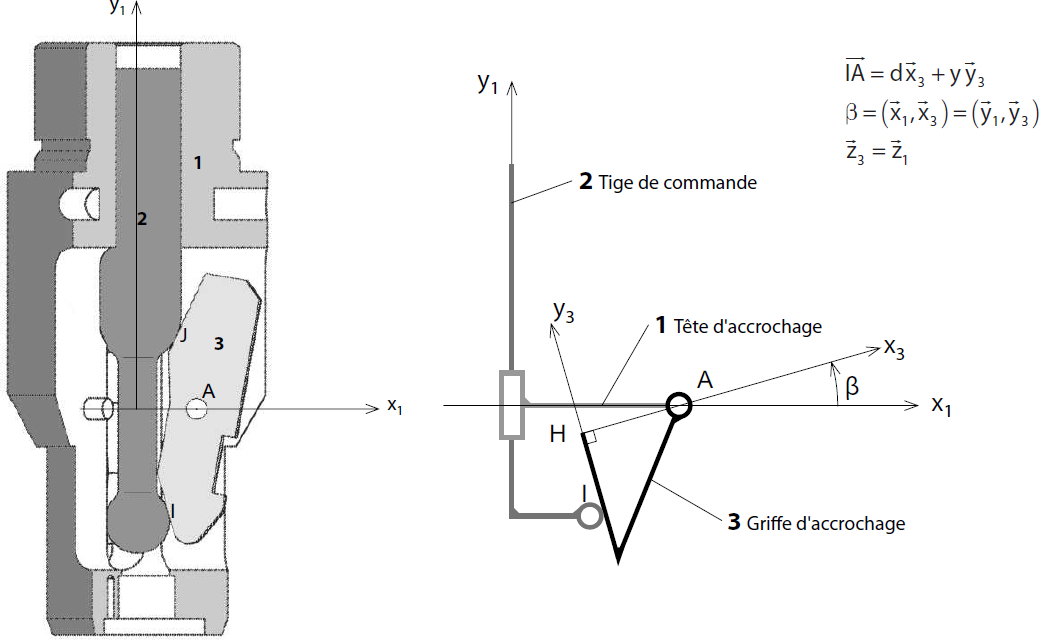
\includegraphics[width=.6\linewidth]{fig_01}

\textit{Guidage de l'ascenseur.}
\end{center}

%\begin{figure}[!ht]
%\centering
%\begin{tikzpicture}
%
%\node at (0,0) {\includegraphics[height=3.5cm]{\pathfig/tour1a_nb}};
%\node at (4,0) {\includegraphics[height=3.5cm]{\pathfig/tour1b_nb}};
%%\draw[gray!50] (-3,3) grid[step=1mm] (6,-2);
%%\draw[gray!90] (-3,3) grid[step=5mm] (6,-2);
%%\node {$\times$};
%
%\node[fill=white,left] at (-2.2,1) {\footnotesize{Galets}}; 
%\node[fill=white,left] at (1,-2.3) {\footnotesize{Guidage en $A$}}; 
%\end{tikzpicture}
%\caption{Tour de la terreur et guidage de l'ascenseur.}
%\end{figure}

%\begin{center}
%\begin{tabular}{cc}
%\includegraphics[height=4.5cm]{\pathfig/tour1a}&
%\includegraphics[height=4.5cm]{\pathfig/tour1b}
%\end{tabular}
%\end{center}

\subsection*{Cahier des charges\\}

Le diagramme des exigences partiel de la Tour de la terreur est donné figure suivante.


\begin{center}
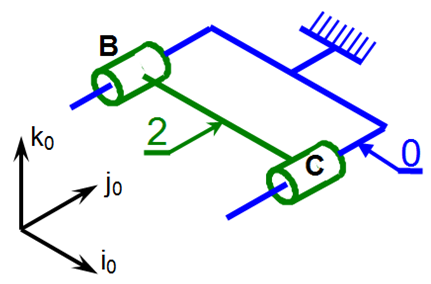
\includegraphics[width=\linewidth]{fig_02}

\textit{Diagramme des exigences partiel.}
\end{center}

%\begin{figure}[!ht]
%\centering
%%\includegraphics{\pathfig/Exigences_Tour}
%\includestandalone[width=.8\linewidth]{\pathfig/Diagramme_exigences_tour}
%\caption{Diagramme des exigences partiel.}
%\label{reqtour}
%\end{figure}

\begin{obj}
L'objectif est d'analyser différentes liaisons en parallèle ou en série de la Tour de la terreur afin de valider l'exigence de précision du guidage lors de la descente.
\end{obj}


%\textcolor{red}{DV : mettre des dimensions h en hauteur et L en largeur}


\begin{center}
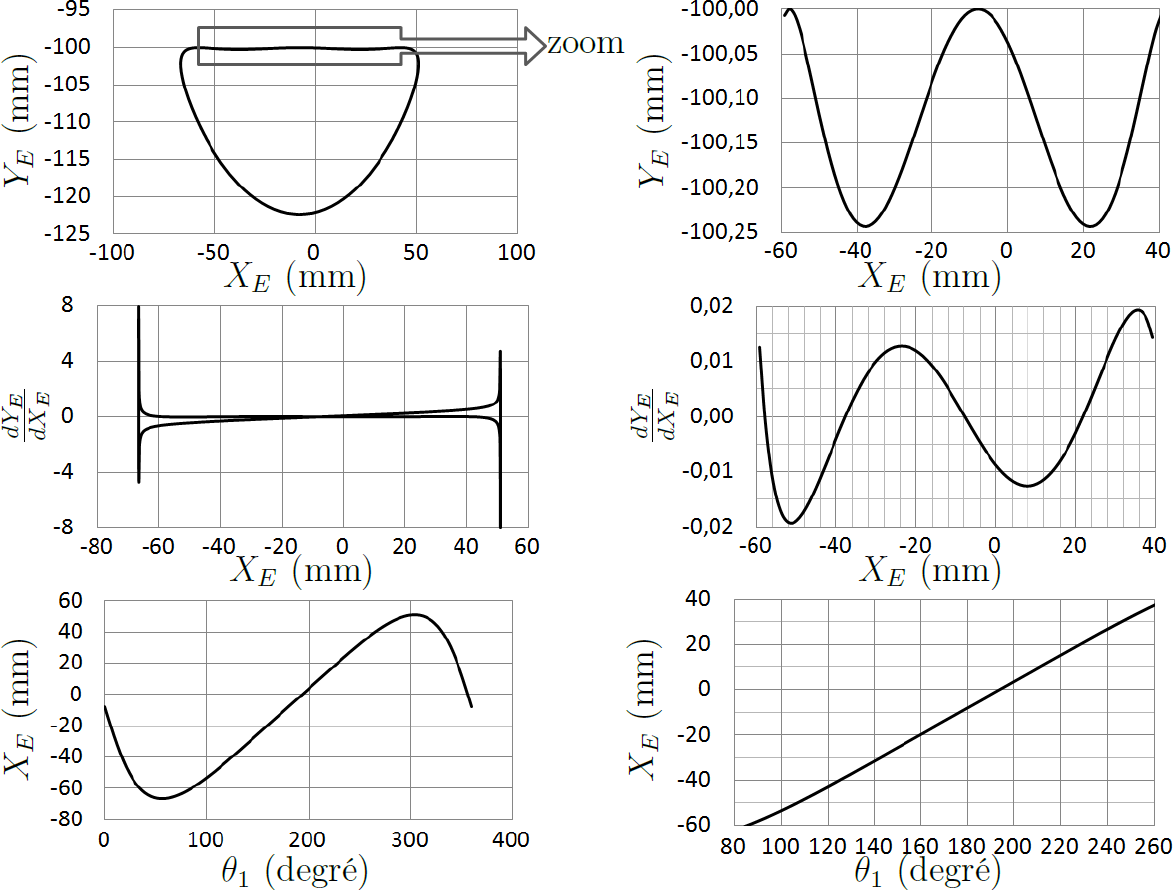
\includegraphics[width=\linewidth]{fig_03}

\textit{Modélisation de la Tour.}
\end{center}

%
%\bigskip
%\noindent
%%\includegraphics[height=7cm]{\pathfig/tour2a.pdf}\hfill
%\includegraphics[height=7cm]{\pathfig/tour2a.png}\hfill
%\begin{tikzpicture}
%%\node (i) {\includegraphics[height=7cm]{\pathfig/tour2b.pdf}};
%\node (i) {\includegraphics[height=7cm]{\pathfig/tour2b.png}};
%\coordinate (o) at (i.south west);
%\draw[->,>=latex] (o) -- ++(1,0) node[right] {$\vect y$};
%\draw[->,>=latex] (o) node[below left] {$O$} -- ++(0,1) node[left] {$\vect z$};
%\draw [latex-latex] (2.5,-1.8) --++(0,2.4) node [right,midway] {$h$};
%\draw [latex-latex] (-1.1,-1.8) --++(3.3,0) node [above,midway] {$L$};
%\end{tikzpicture}
%\captionof{figure}{Modélisation de la Tour.}
%
%
%\piccaption{Association en série d'une liaison pivot et d'une liaison  ponctuelle.\label{SeriePivotPonctuelle}}
%\parpic[r]{\includestandalone{\pathfig/PonctuelleEtPivotSerie}}

On modélise chaque contact entre un galet et le rail par une liaison 
ponctuelle.  On modélise chaque liaison entre un galet et la cabine par une liaison pivot.

Afin de simplifier l'étude, nous nous intéressons d'abord à la liaison équivalente à une liaison pivot en série avec une liaison ponctuelle (liaison réalisée entre la cabine et un rail par l'intermédiaire d'un seul galet).

\begin{center}
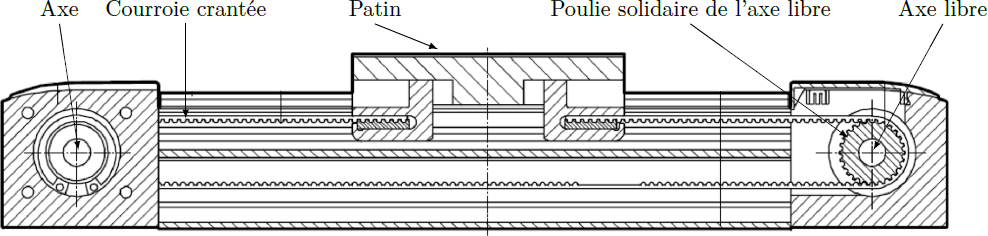
\includegraphics[width=.6\linewidth]{fig_04}

\textit{Association en série d'une liaison pivot et d'une liaison  ponctuelle.}
\end{center}

%
%%\begin{figure}[htbp!]
%%%\includegraphics[width=0.3\textwidth]{\pathfig/PonctuelleEtPivotSerie.png}
%%\caption{}
%%\label{SeriePivotPonctuelle}
%%\end{figure}
%\vspace{1.5cm}}

\question{En utilisant le modèle de la figure précédente,
    montrer que l'association en série d'une ponctuelle de normale
    $\vect{n}$ et d'une liaison pivot d'axe $\vect{z}$ est équivalente à
    une liaison ponctuelle de normale $\vect{n}$.}

Dans la suite, nous considérerons cette simplification pour tous les galets.

\question{Proposer un graphe des liaisons faisant intervenir les modèles des 12 galets entre le rail et l'ascenseur.}

\question{Donner le torseur cinématique d'une liaison ponctuelle ou sphère-plan en précisant le point d'écriture et la base.}

\question{Montrer que l'association de trois liaisons ponctuelles en parallèle au niveau d'un guidage ($A$, $B$, $C$ ou $D$) est équivalente à une liaison sphère-cylindre dont on précisera les caractéristiques.}

\question{Montrer que l'association en parallèle de deux liaisons sphère-cylindre de même axe est équivalente à une liaison pivot glissant.}

%\newpage
%\enlargethispage{\baselineskip}

\question{Conclure sur la liaison équivalente entre la cabine et le rail compte tenu des résultats précédents.}

\question{Pourquoi utilise-t-on cette solution pour guider la cabine de l'ascenseur ?}




\subsection*{Mât réacteur A320}
\setcounter{exo}{0}
 L’étude porte sur la solution d’assemblage choisie entre le mât-réacteur et l’aile de l’avion A320. Les figures suivantes présentent les différentes pièces de cet assemblage ainsi que la disposition des liaisons dans le plan $(\vect{X}, \vect{Z})$.
 
 
\begin{center}
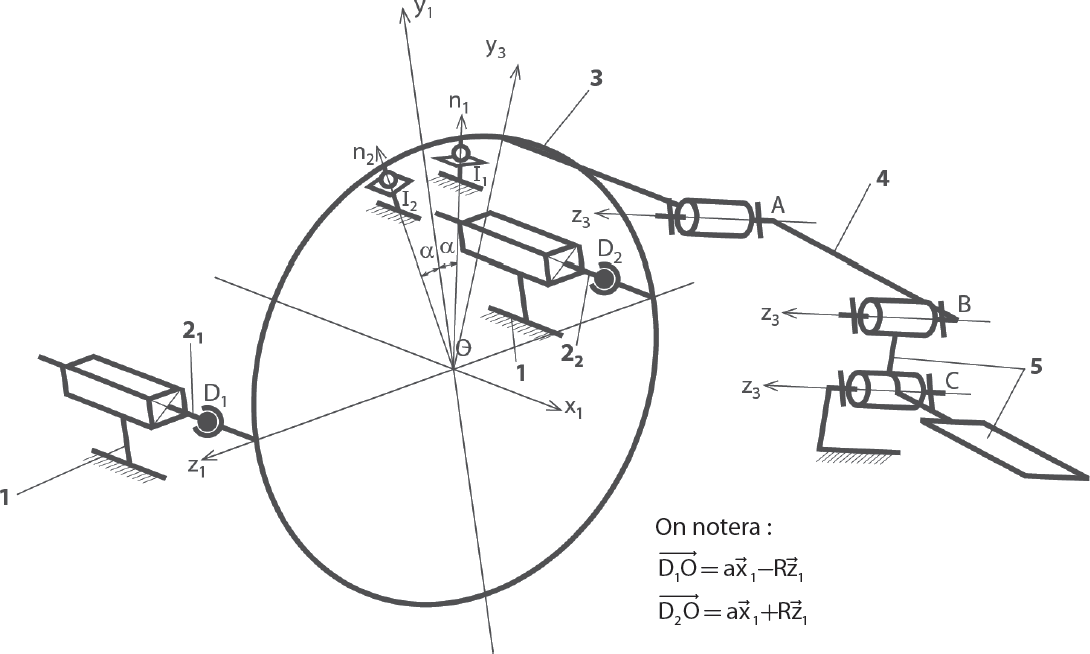
\includegraphics[width=.95\linewidth]{fig_05}
\end{center}

\begin{center}
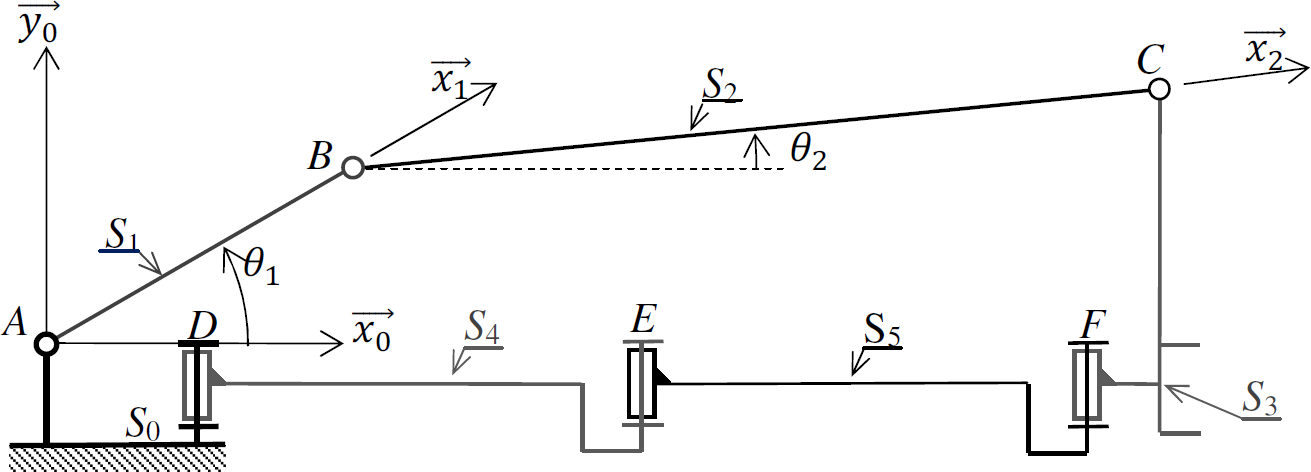
\includegraphics[width=.95\linewidth]{fig_06}
\end{center}

Le mât-réacteur \textbf{(1)} est suspendu à l’aile \textbf{(0)} grâce aux deux biellettes \textbf{(4)} et \textbf{(5)}.
Les articulations réalisées aux points $A$, $B$, $N$ et $M$ sont considérées comme des liaisons << sphériques >>. On a : $\vect{AM}=\vect{BN}=a\vect{z}$ .
Les mouvements du mât-réacteur \textbf{(1)} par rapport à l’aile \textbf{(0)} sont stoppés par la présence de deux triangles \textbf{(2)} et \textbf{(3)}. Le triangle \textbf{(2)} est articulé sur \textbf{(1)} par deux liaisons « shériques » de centres $E$ et $F$, et sur \textbf{(0)} par une liaison « sphérique » de centre $H$. On a : $\vect{EF}=e\vect{y}$ et $\vect{EH}=\dfrac{1}{2}e\vect{y}+h\vect{z}$.

Le triangle \textbf{(3)} est articulé sur \textbf{(1)} par deux liaisons « shériques » de centres $C$ et $D$, et sur \textbf{(0)} par une liaison « sphérique » de centre $J$. On a : $\vect{CD}=a\vect{y}$  et  $\vect{CJ}=\dfrac{1}{2}c\vect{y}-j\vect{x}$.

\question{Tracer le graphe de structure de l’assemblage.}

\question{Déterminer la liaison équivalente entre \textbf{(1)} et \textbf{(0)} réalisée par la biellette \textbf{(4)} puis par la biellette \textbf{(5)}.}

\question{Déterminer la liaison équivalente réalisée entre \textbf{(1)} et \textbf{(0)} par le triangle \textbf{(2)} puis par le triangle \textbf{(3)}.}

\question{Tracer en perspective le schéma architectural de l’assemblage du mât \textbf{(1)} sur l’aile \textbf{(0)} en utilisant les modèles des liaisons équivalentes déterminées aux questions précédentes.}

\question{Déterminer le degré d’hyperstatisme de l’assemblage \textbf{(1)}/\textbf{(0)} ; justifier l’intérêt du résultat en raisonnant sur les dilatations provoquées par des températures et des matériaux différents pour l’aile et le mât-réacteur.}


\fi



\ifprof
\end{multicols}
\else
\end{multicols}
\fi

\ifprof
 
\begin{center}
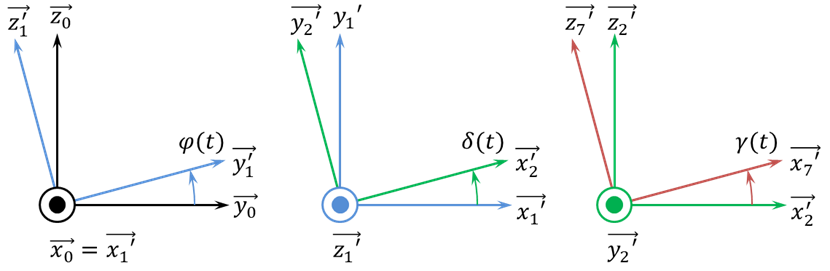
\includegraphics[width=.7\linewidth]{cor_01}
\end{center}

\begin{center}
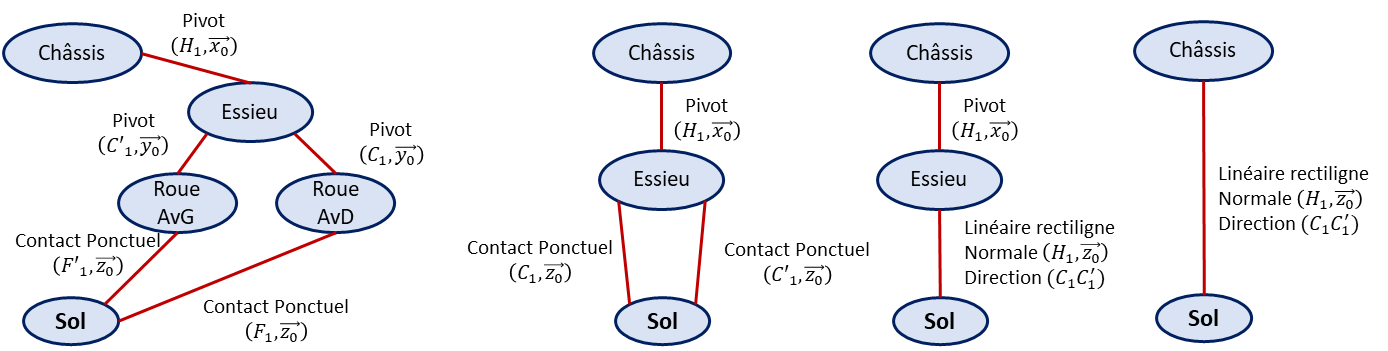
\includegraphics[width=.95\linewidth]{cor_02}
\end{center}

\begin{center}
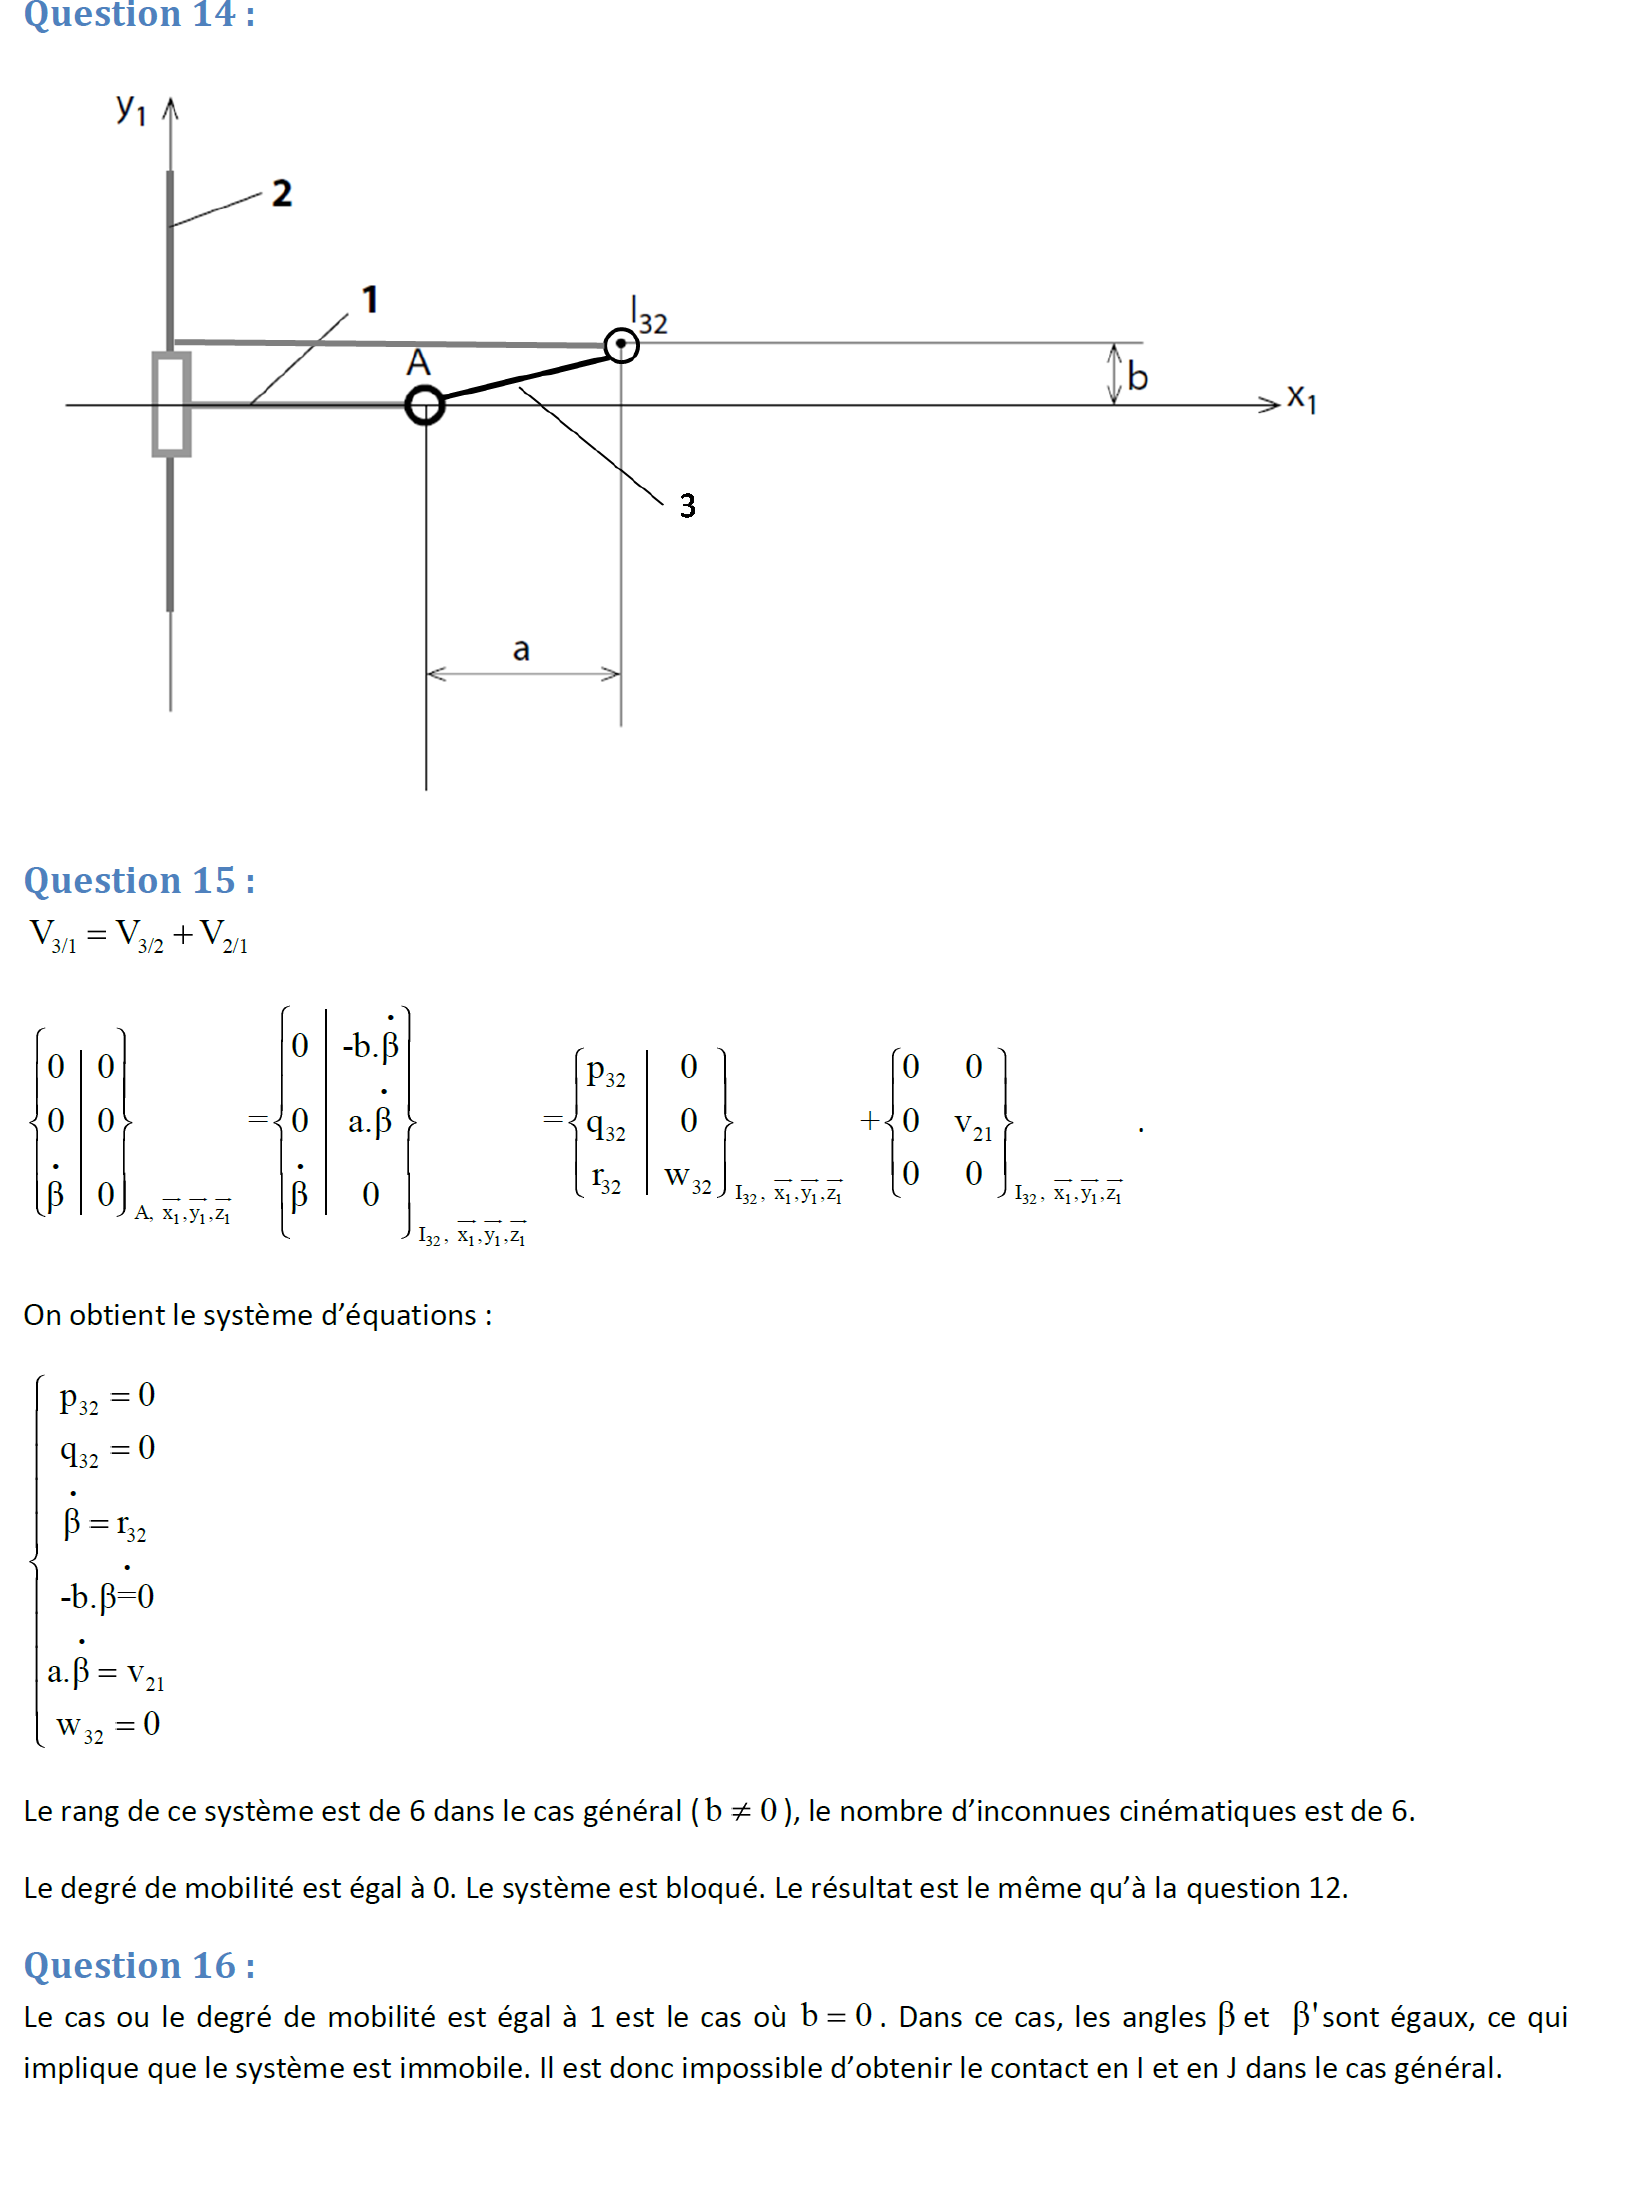
\includegraphics[width=.95\linewidth]{cor_03}
\end{center}

\begin{center}
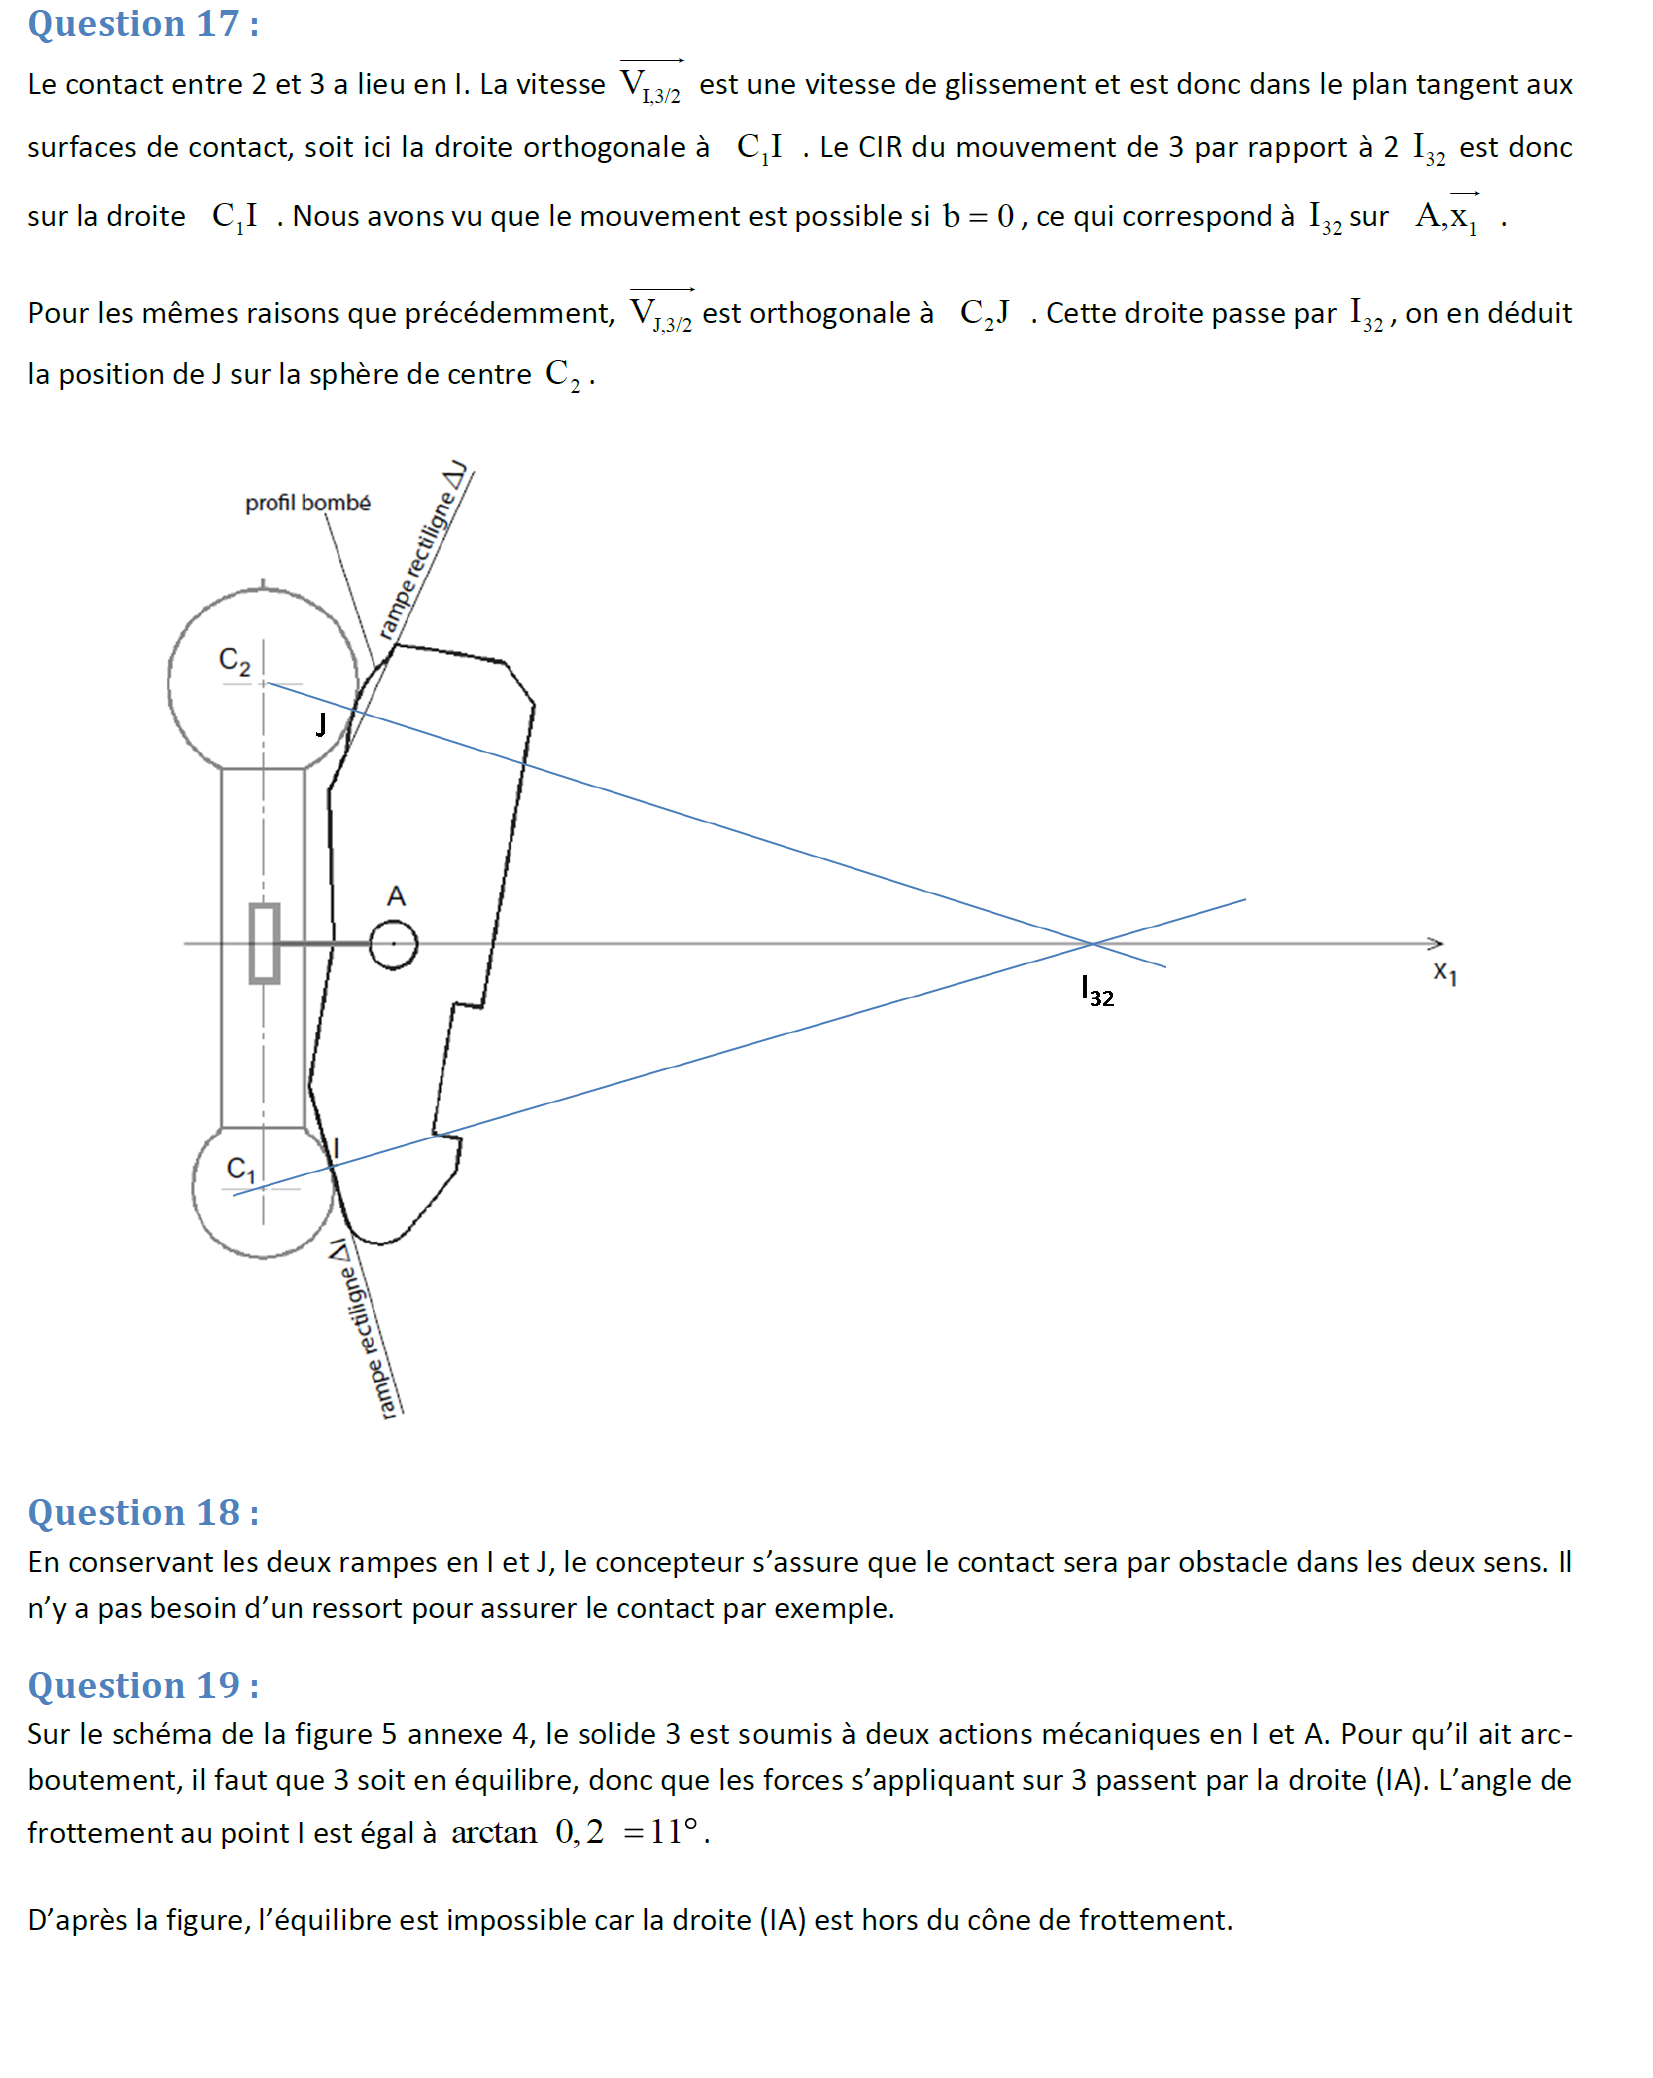
\includegraphics[width=.95\linewidth]{cor_04}
\end{center}

\else
\fi